\chapter{Background}


\section{Past Solution}

On the NASA space challenge website, many participants had offered their solution 
by machine learning or performed prediction/verification using flight timetables 
and routes. However, these methods usually only can be used to find the existence 
of contrails, or the possibility of that those contrails exist. Meanwhile, it 
really relies on the flight data and the photo location, but it is not feasible
for scientists to access all the flight database.

Here are some examples of the solutions propoised:
\begin{itemize}
\item \href{https://2016.spaceappschallenge.org/challenges/aero/clouds-or-contrails/projects/contrailers-exeter}{Contrailers-Exeter} \\
This team mentioned in their explanation that they determine the probability 
of contrails by examining recent flights in the area and the air temperature. 
\item \href{https://2016.spaceappschallenge.org/challenges/aero/clouds-or-contrails/projects/hot-on-the-contrail}{Hot on the Contrail}\\
This team proposes a machine learning solution, however, they only determine 
the possibility of contrails existing, but not where the contrails actually are. 
This solution has been proposed for the NASA space challenge, but it seems not 
to be useful for detecting the actual contrails locations.  
\end{itemize}

\section{Aim and Target}

In order for scientists to do better research on contrails and clouds, 
the aim of this project proposes a program to automatically segment the 
contrails from clouds on different kinds of images, such as satellites 
images, photos, and so on. After the contrails in the image have been 
determined, they are highlighted and a comparison image is output.

\section{Scope and Constraints}
In this section, we outline some constraints exhibited by our approach and give
the scope of our work.

Our project can not use images with interference information, an example is shown
in Figure |ref{figure1}, which has latitude and longitude lines and map boards. 
These lines are much clearer than cloud outlinesn the images and they will 
disrupt the detection result.
\begin{figure}[htb!]
\centering
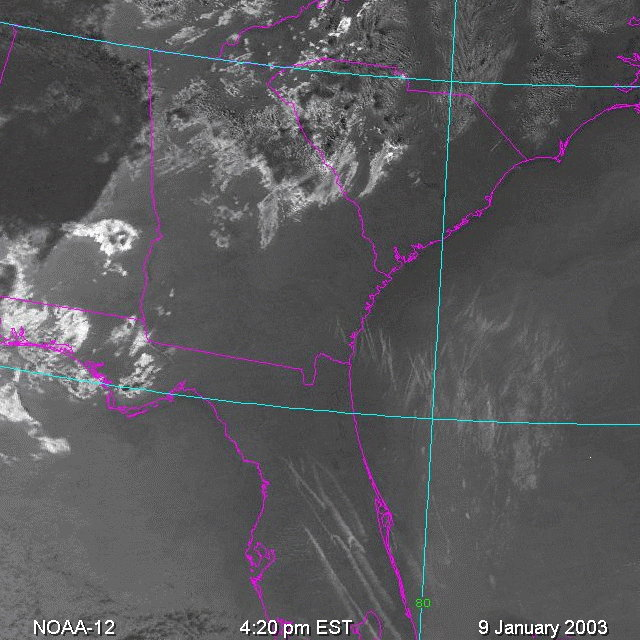
\includegraphics[scale=0.5]{pic/figure1.jpg}
\caption[Short form for the mapping directory]{"figure1.jpg"}
\label{figure1}
\end{figure}
Our program is inefficient for processing large images. The 
strategical removal of non-line edgels is computationally expensive.
